\begin{center}
\Huge
Arealer mellem grafer
\end{center}

\section*{Arealer mellem grafer}
\stepcounter{section}

Skal vi bestemme arealet mellem graferne for to funktioner $f$ og $g$ på et interval $[a,b]$, og funktionerne begge er positive på hele intervallet, så er det meget naturligt først at finde arealet under den øverste, lad os sige $f$, og efterfølgende trække arealet under den nederste fra. Dette er visualiseret på Figur \ref{fig:arealmellemgrafer}, og kan bestemmes som integralet
\begin{align*}
	A = \int_a^b f(x) - g(x) dx,
\end{align*}
og det viser sig faktisk, at man kan bestemme arealet mellem graferne for $f$ og $g$ på intervallet $[a,b]$ på denne vis 
uagtet om funktionerne $f$ og $g$ er positive på intervallet eller ej. 
\begin{figure}[H]
	\centering
	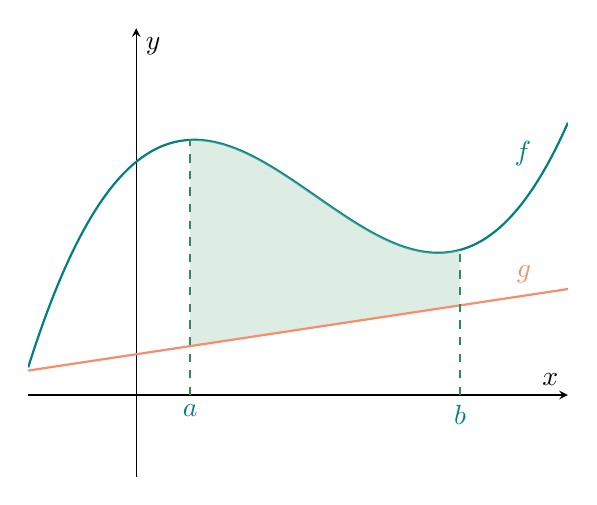
\begin{tikzpicture}
	\begin{axis}[
		axis lines = center, xmin = -2, xmax = 8,
		ymin = -1, ymax = 4.5,
		ticks = none, 
		xlabel = $x$,
		ylabel = $y$,
		]
			\addplot[color = teal, domain = -2:8, samples = 500, thick] {0.03*x^(3) - 0.3*x^(2) + 0.54*x + 2.86};
			\fill[color = SeaGreen!40, variable = \x, domain = 1:6,opacity = 0.4] 
			 plot (axis cs: \x, 0.03*\x^3 - 0.3*\x^2 + 0.54*\x + 2.86) --
			 plot[domain = 6:1] (axis cs: \x, 0.1*\x + 0.5) --
			 cycle;
			 \addplot[color = Melon, domain = -2:8, thick] {0.1*x + 0.5};
			 \draw[color = SeaGreen, dashed, thick] (axis cs: 1,0) -- (axis cs: 1,3.14);
			 \draw[color = SeaGreen, dashed, thick] (axis cs: 6,0) -- (axis cs: 6,1.78);
			 \node[color = teal, anchor = north] at (axis cs: 1,0) {$a$};
			 \node[color = teal, anchor = north] at (axis cs: 6,0) {$b$};
			 \node[color = teal, anchor = south east] at (axis cs: 7.5,2.69) {$f$};
			 \node[color = Melon, anchor = south east] at (axis cs: 7.5,1.25) {$g$};
	\end{axis}
	\end{tikzpicture}
	\caption{Areal mellem grafer for positive funktioner $f$ og $g$}
	\label{fig:arealmellemgrafer}
\end{figure}
Vi har for funktioner $f$ og $g$ følgende resultat, vi kan anvende - også hvis $f$ og $g$ ikke er nødvendigvis er positive på intervallet.
Til dette får vi dog brug for følgende sætning.
\newpage
\begin{setn}
	\label{setn:hjælp}
	For to kontinuerte funktioner $f$ og $g$ samt konstanter $c \in \mathbb{R}$ har vi, at 
	\begin{align*}
		\int_a^bf(x) + g(x) dx = \int_a^b f(x) dx + \int_a^b g(x) dx
	\end{align*}
	og
	\begin{align*}
		\int_a^b cf(x) dx = c\int_a^b f(x) dx.
	\end{align*}
\end{setn}
\begin{proof}
	Vi har
	\begin{align*}
		\int_a^b f(x) + g(x) dx &= F(b) + G(b) -(F(a) + G(a)) \\
		&= F(b) + G(b) - F(a) - G(a) \\
		&= F(b) - F(a) + G(b) - G(a) \\
		&= \int_a^b f(x) dx + \int_a^b g(x) dx, 
	\end{align*}
	og 
	\begin{align*}
		\int_a^b cf(x) dx &= (cF(b)-cF(a)) \\
		 &= c(F(b)-F(a)) \\
		 &= c\int_a^b f(x) dx.
	\end{align*}
\end{proof}
\begin{setn}[Arealer mellem grafer]\label{setn:hovedsætn}
	Lad $f$ og $g$ være kontinuerte på intervallet $[a,b]$ samt lad $f(x) \geq g(x)$ for alle $x \in [a,b]$. Arealet $A$ af
	punktmængden afgrænset af graferne $f$ og $g$ på intervallet $[a,b]$ er så givet ved
	\begin{align*}
		A = \int_a^b f(x) - g(x) dx.	
	\end{align*}	 
\end{setn}
\begin{proof}
	Vi parallelforskyder graferne for $f$ og $g$ langs $y$-aksen indtil både $f$ og $g$ er positive på hele $[a,b]$. 
	Dette tilsvarer at lægge et tal $k$ til begge funktioner $f$ og $g$. Vi kan se forskydningen på Figur 
	\ref{fig:parallelop}.
	\begin{figure}[H]
	\centering
		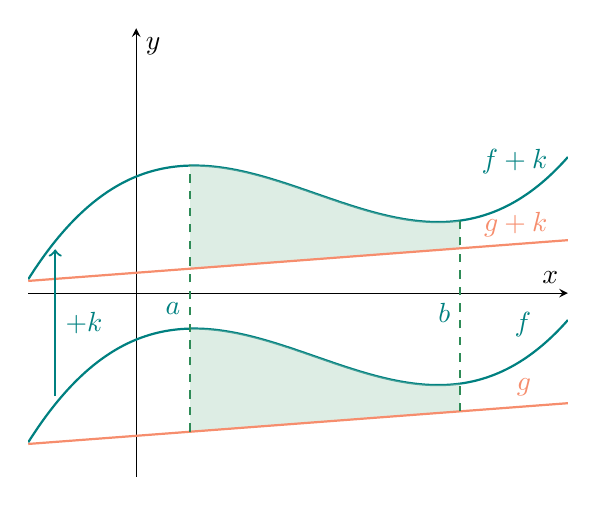
\begin{tikzpicture}
		\begin{axis}[
		axis lines = center, xmin = -2, xmax = 8,
		ymin = -4.5, ymax = 6.5,
		ticks = none, 
		xlabel = $x$,
		ylabel = $y$,
		]
			\addplot[color = teal, domain = -2:8, samples = 500, thick] {0.03*x^(3) - 0.3*x^(2) + 0.54*x + 2.86};
			\fill[color = SeaGreen!40, variable = \x, domain = 1:6,opacity = 0.4] 
			 plot (axis cs: \x, 0.03*\x^3 - 0.3*\x^2 + 0.54*\x + 2.86) --
			 plot[domain = 6:1] (axis cs: \x, 0.1*\x + 0.5) --
			 cycle;
			 \addplot[color = Melon, domain = -2:8, thick] {0.1*x + 0.5};
			 \addplot[color = teal, domain = -2:8, samples = 500, thick] {0.03*x^(3) - 0.3*x^(2) + 0.54*x + 2.86 - 4};
			\fill[color = SeaGreen!40, variable = \x, domain = 1:6,opacity = 0.4] 
			 plot (axis cs: \x, 0.03*\x^3 - 0.3*\x^2 + 0.54*\x + 2.86 - 4) --
			 plot[domain = 6:1] (axis cs: \x, 0.1*\x + 0.5-4) --
			 cycle;
			 \addplot[color = Melon, domain = -2:8, thick] {0.1*x + 0.5-4};
			 \draw[color = SeaGreen, dashed, thick] (axis cs: 1,-3.4) -- (axis cs: 1,3.14);
			 \draw[color = SeaGreen, dashed, thick] (axis cs: 6,-2.9) -- (axis cs: 6,1.78);
			 \node[color = teal, anchor = north east] at (axis cs: 1,0) {$a$};
			 \node[color = teal, anchor = north east] at (axis cs: 6,0) {$b$};
			 \node[color = teal, anchor = south east] at (axis cs: 7.8,2.69) {$f + k$};
			 \node[color = Melon, anchor = south east] at (axis cs: 7.8,1.15) {$g + k$};
			 \node[color = teal, anchor = south east] at (axis cs: 7.5,2.69-4) {$f$};
			 \node[color = Melon, anchor = south east] at (axis cs: 7.5,1.25-4) {$g$};
			 \draw[->,color = teal, thick] (axis cs: -1.5,-2.52625) -- (axis cs: -1.5,1.07375)
			 node[midway, anchor = west] {$+k$};
		\end{axis}
		\end{tikzpicture}
		\caption{Parallelforskydning langs $y$-aksen af graferne for $f$ og $g$.}
		\label{fig:parallelop}
	\end{figure}
	Vi kan af Figur \ref{fig:parallelop} se, at arealerne mellem graferne ikke ændrer sig, når vi parallelforskyder 
	graferne for $f$ og $g$ med en konstant $k$ langs $y$-aksen. Vi bestemmer derfor arealet mellem de parallelforskudte 
	funktioner. Bemærk, at vi her anvender Sætning \ref{setn:hjælp}.
	\begin{align*}
		A &= \int_a^b f(x) + k dx - \int_a^bg(x) + k dx \\
		&= \int_a^b f(x) + k - (g(x) + k) dx \\
		&= \int_a^b f(x) +k - g(x) - k dx \\
		&= \int_a^b f(x) - g(x) dx   
	\end{align*}
\end{proof}
Det er altså helt ligegyldigt om graferne for funktionerne lægger under $x$-aksen. Når vi skal bestemme arealet mellem dem, så bestemmer vi blot det bestemte integral af deres forskel. Lad os se, hvordan vi kan anvende denne sætning til at bestemme arealet mellem graferne for to funktioner. 
\begin{exa}
	Vi betragter graferne for funktionerne $f$ og $g$ givet ved henholdsvis
	\begin{align*}
		f(x) = -x^2 + x + 6
	\end{align*}
	 og 
	 \begin{align*}
	 	g(x) = x + 2.
	 \end{align*}
	 Graferne samt det ønskede areal kan ses på Figur \ref{fig:exa}
	 \begin{figure}[H]
	\centering
		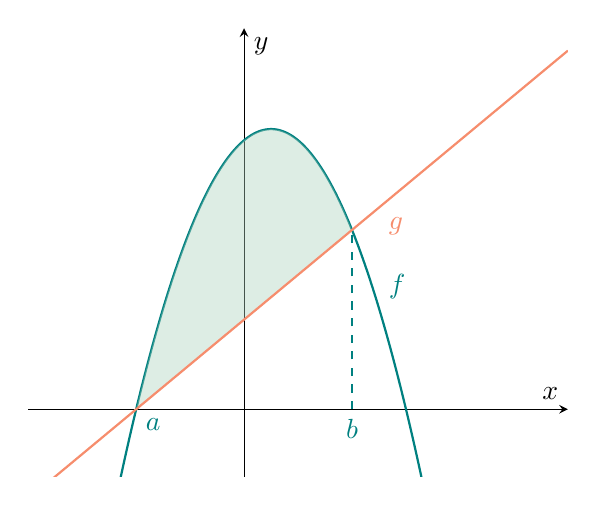
\begin{tikzpicture}
		\begin{axis}[
		axis lines = center, xmin = -4, xmax = 6,
		ymin = -1.5, ymax = 8.5,
		ticks = none, 
		xlabel = $x$,
		ylabel = $y$,
		]
			\addplot[color = teal, domain = -4:6, samples = 500, thick] {-x^2 + x + 6};
			\fill[color = SeaGreen!40, variable = \x, domain = -2:2,opacity = 0.4] 
			plot (axis cs: \x, {- 1.0*(\x)^2 + \x + 6}) --
			plot[domain = 2:-2] (axis cs: \x, {\x + 2}) --  cycle;			 
			 \addplot[color = Melon, domain = -4:6, thick] {x + 2};
			 \node[color = Melon, anchor = north west] at (axis cs: 2.5,4.5) {$g$};
			 \node[color = teal, anchor = south west] at (axis cs: 2.5,2.25) {$f$};
			 \node[color = teal, anchor = north west] at (axis cs: -2,0) {$a$};
			 \node[color = teal, anchor = north] at (axis cs: 2,0) {$b$};
			 \draw[color = teal, thick, dashed] (axis cs: 2,0) -- (axis cs:2, 4);
		\end{axis}
		\end{tikzpicture}
		\caption{Areal afgrænset af graferne for $f$ og $g$.}
		\label{fig:exa}
	\end{figure}
	For at bestemme arealet mellem graferne for $f$ og $g$, skal vi først bestemme intervalendepunkterne $a$ og $b$. 
	Disse kaldes for \textit{øvre} og \textit{nedre grænse} for integralet. Vi sætter altså funktionerne lig hinanden.
	\begin{align*}
		f(x) = g(x) \ &\Leftrightarrow \ -x^2 + x + 6 = x + 2 \\
		&\Leftrightarrow \ -x^2 = -4 \\
		&\Leftrightarrow \ x = \pm 2.
	\end{align*}
	Arealet er altså givet ved følgende integral.
	\begin{align*}
		\int_{a}^bf(x) - g(x) &= \int_{-2}^2 -x^2 + x + 6 -(x + 2) dx \\
		&= \int_{-2}^2 -x^2 +4 dx \\
		&= \left[-\frac{1}{3}x^3 + 4x\right]_{-2}^2 \\
		&= -\frac{1}{3}2^3 + 4\cdot 2 - \left(-\frac{1}{3}(-2)^3 + 4(-2)\right)\\
		&= -\frac{8}{3} + 8 - \frac{8}{3} + 8 \\
		&= -\frac{16}{3} + \frac{48}{3} \\
		&= \frac{32}{3} 
	\end{align*}
	Arealet er derfor givet ved $\frac{32}{3}$.
\end{exa}
\newpage
Vi får brug for følgende to sætninger, der er lette at bevise.
\begin{setn}\label{setn:1}
	For en funktion $f$, der er negativ på intervallet $[a,b]$ er arealet $A$ mellem grafen for $f$ og $x$-aksen på 
	intervallet $[a,b]$ givet ved
	\begin{align*}
		A = -\int_a^bf(x) dx
	\end{align*}
\end{setn}
\begin{proof}
	Opgave.
\end{proof}
\begin{setn}\label{setn:2}
	For $a,b,c\in \mathbb{R}$, hvor $a < b < c$ og en funktion $f$ gælder der, at 
	\begin{align*}
		\int_a^c f(x) dx = \int_a^bf(x) dx + \int_b^c f(x) dx
	\end{align*}
\end{setn}
\begin{proof}
	Opgave.
\end{proof}

\newpage

\subsection*{Opgave 1}

Opskriv det markerede areal på Figur \ref{fig:opg1} ved integraler. Du skal ikke udregne integralerne. 
\begin{figure}[H]
	\centering
		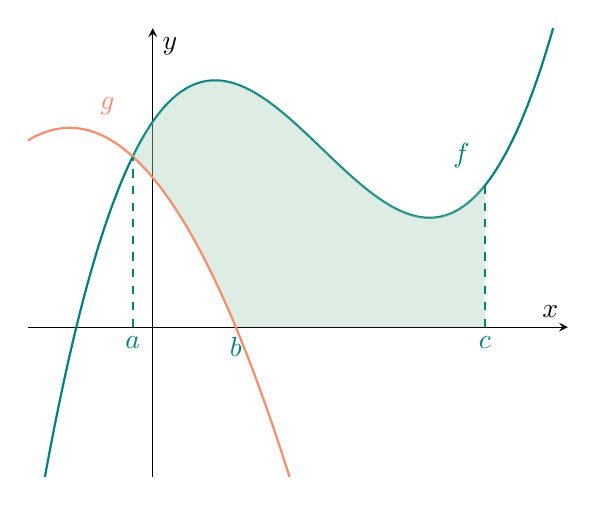
\begin{tikzpicture}
		\begin{axis}[
		axis lines = center, xmin = -3, xmax = 10,
		ymin = -3, ymax = 6,
		ticks = none, 
		xlabel = $x$,
		ylabel = $y$,
		]
			\addplot[color = teal, domain = -3:10, samples = 500, thick] {0.04*x^(3) - 0.49*x^(2) + 1.2*x + 4.12};
			\fill[color = SeaGreen!40, variable = \x, domain = -0.482:8,opacity = 0.4] 
			plot (axis cs: \x, {0.04*(\x)^3 - 0.49*(\x)^2 + 1.2*\x + 4.12}) --
			(axis cs: 8,0) --
			plot[domain = 2:-0.482] (axis cs: \x, {-0.25*(\x)^2 - \x + 3}) --
			 cycle;			 
			 \addplot[color = Melon, domain = -4:6, thick, samples = 500] {-0.25*x^2 - x + 3};
			 \node[color = Melon, anchor = north west] at (axis cs: -1.5,4.8) {$g$};
			 \node[color = teal, anchor = south west] at (axis cs: 7,3) {$f$};
			 \node[color = teal, anchor = north] at (axis cs: -0.482,0) {$a$};
			 \node[color = teal, anchor = north] at (axis cs: 2,0) {$b$};
			  \node[color = teal, anchor = north] at (axis cs: 8,0) {$c$};
			 \draw[color = teal, thick, dashed] (axis cs: -0.482,0) -- (axis cs:-0.482, 3.424);
			 \draw[color = teal, thick, dashed] (axis cs: 8,0) -- (axis cs:8, 2.84);
		\end{axis}
		\end{tikzpicture}
		\caption{Markeret areal.}
		\label{fig:opg1}
	\end{figure}

\subsection*{Opgave 2}

Opskriv det markerede areal på Figur \ref{fig:opg2} ved integraler. Du skal ikke udregne integralerne 
\begin{figure}[H]
	\centering
		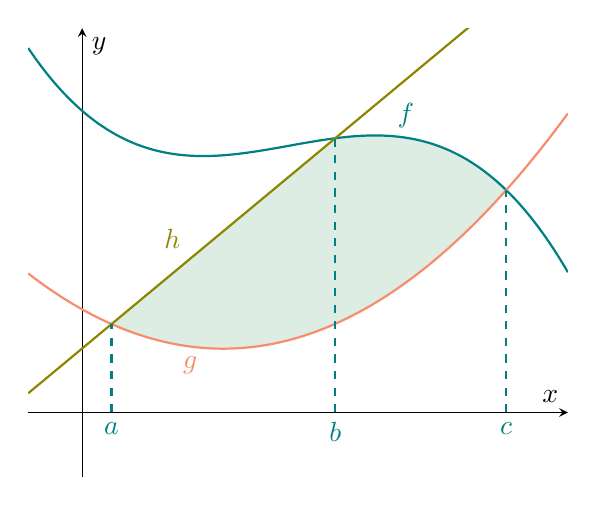
\begin{tikzpicture}
		\begin{axis}[
		axis lines = center, xmin = -1, xmax = 9,
		ymin = -1, ymax = 6,
		ticks = none, 
		xlabel = $x$,
		ylabel = $y$,
		]
			
			\fill[color = SeaGreen!40, variable = \x,opacity = 0.4] 
			plot[domain = 0.544: 4.689] (axis cs: \x, {0.7*\x + 1}) --
			plot[domain = 4.689: 7.856] (axis cs: \x, {-0.02*(\x)^(3) + 0.23*(\x)^(2) - 0.73*\x + 4.71}) --
			plot[domain = 7.856:0.544] (axis cs: \x, {0.09*(\x)^(2) - 0.47*\x + 1.61}) --
			 cycle;			 
			 \addplot[color = teal, domain = -1:9, samples = 500, thick] {-0.02*x^(3) + 0.23*x^(2) - 0.73*x + 4.71};
			 \addplot[color = Melon, domain = -1:9, thick, samples = 500] {0.09*x^(2) - 0.47*x + 1.61};
			 \addplot[color = olive, domain = -1:9, samples = 500, thick] {0.7*x+1};
			 \node[color = teal, anchor = south] at (axis cs: 6,4.29) {$f$};
			 \node[color = Melon, anchor = north] at (axis cs: 2,1.03) {$g$};
			 \node[color = olive, anchor = south east] at (axis cs: 2,2.4) {$h$};
			 \node[color = teal, anchor = north] at (axis cs: 0.544,0) {$a$};
			 \node[color = teal, anchor = north] at (axis cs: 4.689,0) {$b$};
			  \node[color = teal, anchor = north] at (axis cs: 7.856,0) {$c$};
			 \draw[color = teal, thick, dashed] (axis cs: 0.544,0) -- (axis cs:0.544, 1.381);
			 \draw[color = teal, thick, dashed] (axis cs: 4.689,0) -- (axis cs:4.689,4.282);
			 \draw[color = teal, thick, dashed] (axis cs: 7.856,0) -- (axis cs:7.856,3.473);
		\end{axis}
		\end{tikzpicture}
		\caption{Areal afgrænset af graferne for $f$ og $g$.}
		\label{fig:opg2}
	\end{figure}
	
\newpage

\subsection*{Opgave 3}
Graferne for to funktioner $f$ og $g$ givet ved henholdsvis
\begin{align*}
	f(x) = -2x + 3
\end{align*}
og 
\begin{align*}
	g(x) = x -1
\end{align*}
kan ses på Figur \ref{fig:opg3}.
\begin{enumerate}[label=\roman*)]
	\item Bestem arealet af det markerede område på Figur \ref{fig:opg3}.
\end{enumerate}
\begin{figure}[H]
	\centering
	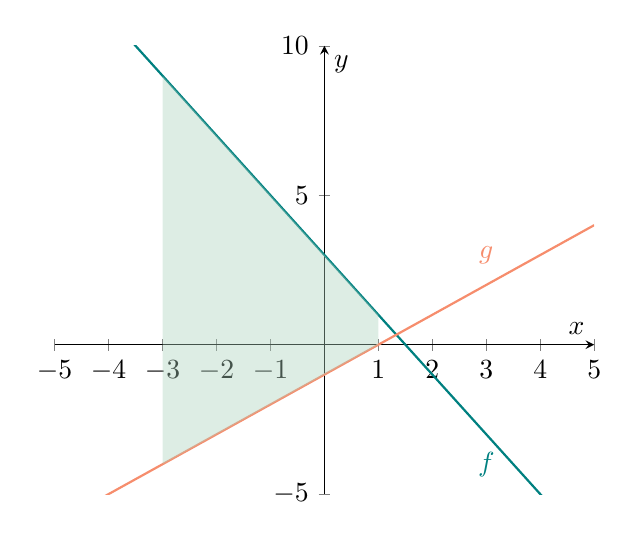
\begin{tikzpicture}
	\begin{axis}[
		axis lines = center, 
		xmin = -5, xmax = 5,
		ymin = -5, ymax = 10,
		xtick = {-5,-4,-3,...,3,4,5},
		xlabel = $x$, 
		ylabel = $y$, 
	]
		\addplot[color = teal, thick, domain = -5:5] {-2*x + 3};	
		\addplot[color = Melon, thick, domain = -5:5] {x - 1};			
		\fill
		[
			color = SeaGreen!40,
			opacity = 0.4,
			variable = \x, 
		]	
			plot[domain = -3:1](axis cs: \x, \x - 1) --
			plot[domain = 1:-3](axis cs: \x, -2*\x + 3) -- 
			  cycle;
		\node[color = teal] at (axis cs: 3,-4) {$f$};
		\node[color = Melon] at (axis cs: 3,3) {$g$};
	\end{axis}
	\end{tikzpicture}
	\caption{Areal mellem $f$ og $g$.}
	\label{fig:opg3}
\end{figure}
\newpage
\subsection*{Opgave 4}
Graferne for to funktioner $f$ og $g$ givet ved henholdsvis
\begin{align*}
	f(x) = 0.5x^2 - 4
\end{align*}
og 
\begin{align*}
	g(x) = 3x + 3
\end{align*}
kan ses på Figur \ref{fig:opg4}.
\begin{enumerate}[label=\roman*)]
	\item Bestem arealet af det markerede område på Figur \ref{fig:opg4}.
\end{enumerate}
\begin{figure}[H]
	\centering
	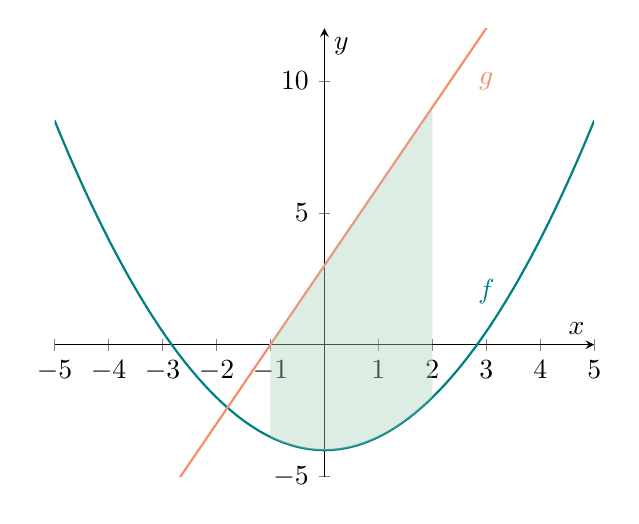
\begin{tikzpicture}
	\begin{axis}[
		axis lines = center, 
		xmin = -5, xmax = 5,
		ymin = -5, ymax = 12,
		xtick = {-5,-4,-3,...,3,4,5},
		xlabel = $x$, 
		ylabel = $y$, 
	]
		\addplot[color = teal, thick, domain = -5:5, samples = 500] {1/2*x^2-4};	
		\addplot[color = Melon, thick, domain = -5:5] {3*x+3};			
		\fill
		[
			color = SeaGreen!40,
			opacity = 0.4,
			variable = \x, 
		]	
			plot[domain = -1:2](axis cs: \x, {0.5*(\x)^2 - 4}) --
			plot[domain = 2:-1](axis cs: \x, {3*\x + 3}) -- 
			  cycle;
		\node[color = teal] at (axis cs: 3,2) {$f$};
		\node[color = Melon] at (axis cs: 3,10) {$g$};
	\end{axis}
	\end{tikzpicture}
	\caption{Areal mellem $f$ og $g$.}
	\label{fig:opg4}
\end{figure}
\newpage

\subsection*{Opgave 5}
Grafen for en funktion $f$ givet ved
\begin{align*}
	f(x) = x^3 - 4 x^2 + x + 6
\end{align*}

kan ses på Figur \ref{fig:opg5}.
\begin{enumerate}[label=\roman*)]
	\item Bestem arealet af det markerede område på Figur \ref{fig:opg5}.
\end{enumerate}
\begin{figure}[H]
	\centering
	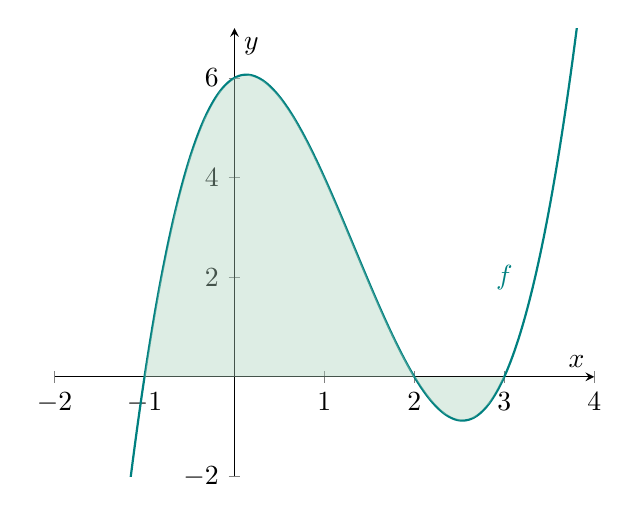
\begin{tikzpicture}
	\begin{axis}[
		axis lines = center, 
		xmin = -2, xmax = 4,
		ymin = -2, ymax = 7,
		xtick = {-5,-4,-3,...,3,4,5},
		xlabel = $x$, 
		ylabel = $y$, 
	]
		\addplot[color = teal, thick, domain = -5:5, samples = 500] {x^3 - 4*x^2 + 1*x + 6};		
		\fill
		[
			color = SeaGreen!40,
			opacity = 0.4,
			variable = \x, 
		]	
			plot[domain = -1:3](axis cs: \x, {(\x)^3 - 4*(\x)^2 + 1*\x + 6}) --
			  cycle;
		\node[color = teal] at (axis cs: 3,2) {$f$};
		\node[color = Melon] at (axis cs: 3,10) {$g$};
	\end{axis}
	\end{tikzpicture}
	\caption{Areal afgrænset af grafen for $f$ og $x$-aksen.}
	\label{fig:opg5}
\end{figure}

\newpage

\subsection*{Opgave 6}
Bestem arealet af området afgrænset af følgende par af funktioner.
\begin{enumerate}[label=\roman*)]
	\item $f(x) = 3x^2-4$ og $g(x) = 2x^2 + 3x$.
	\item $f(x) = x^3$ og $g(x) = x^7$ (Vink: Der er to områder)
	\item $f(x) = 10x - x^2$ og $g(x) = x^2$.
\end{enumerate}

\subsection*{Opgave 7}
Vi skal bevise Sætning \ref{setn:1}.
\begin{enumerate}[label=\roman*)]
	\item Anvend Sætning \ref{setn:hovedsætn} hvor $f(x) \equiv 0$.
\end{enumerate}

\subsection*{Opgave 8}
Vi skal bevise Sætning \ref{setn:2}.
\begin{enumerate}[label=\roman*)]
	\item Opskriv
	\begin{align*}
		\int_a^c f(x) dx
	\end{align*} 
	med stamfunktioner og læg $F(b)-F(b)$ til.
	\item Omskriv tilbage til integraltegn.
\end{enumerate}

